\problemname{Door to Treasure
}

Elmo is hunting for pirate treasure. The treasure is locked behind a door which requires a special key to be opened. To obtain this key, Elmo must solve a pirate puzzle involving $N$ keys and $M$ chests. The keys are labelled from 1 to $N$ and the chests are labelled from 1 to $M$. The $N$th key is the special key that will open the door to the treasure.

Each chest contains a single key. Also, each chest requires a non-empty set of keys to unlock it. Once the chest is unlocked, Elmo gets the key inside and can use it as many times as they like in the future. It is possible for two chests to contain duplicate keys. Elmo may start with 0 or more keys in their pocket that can be used to open chests. These pocket keys were previously acquired during Elmo's prior swashbuckling adventures.

\begin{center}
    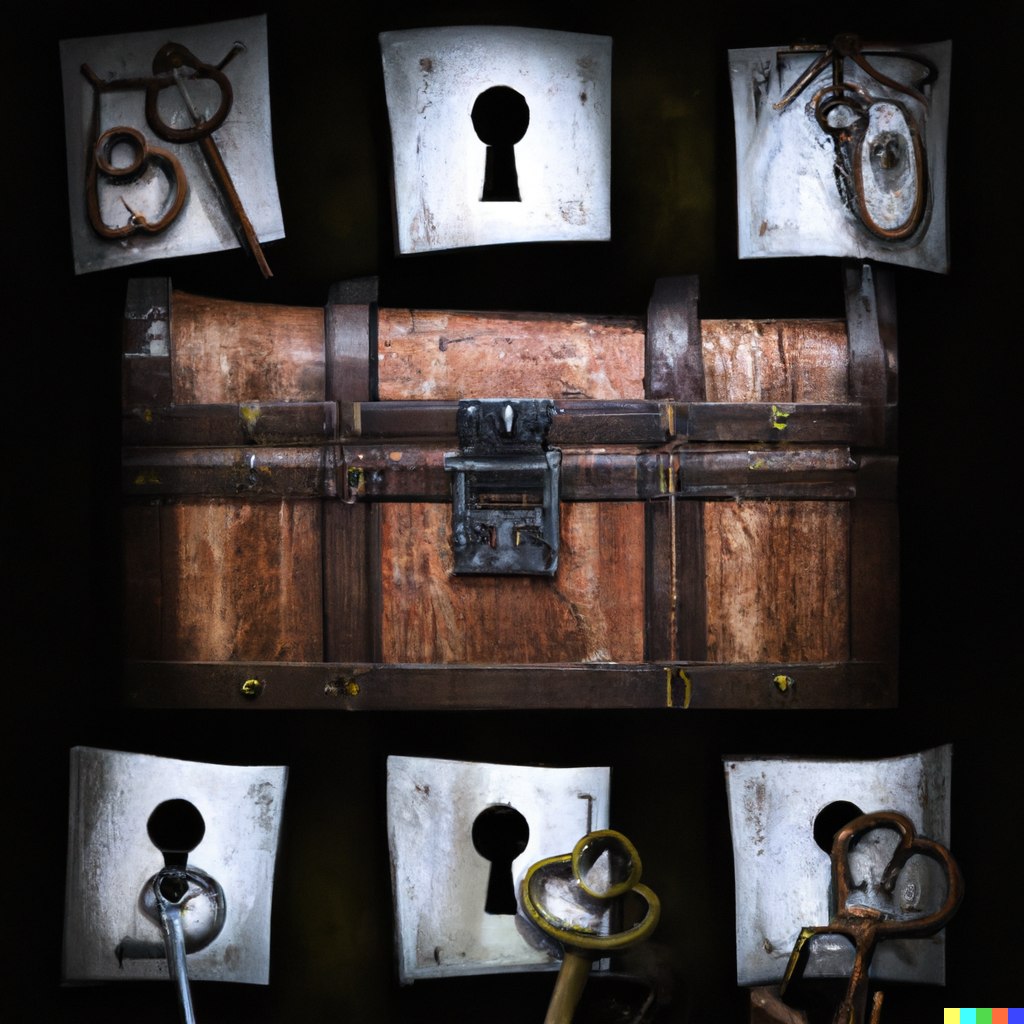
\includegraphics[width=0.4\textwidth]{fig}
\end{center}


Since Elmo does not want to waste time, they want to find an efficient strategy to open the door to the treasure. A strategy is a (possibly empty) set of chests that can be arranged into at least one \textit{valid order} specifying the sequence of chests to unlock. To be a valid order, you must obtain the $N$th key at some point and every chest in the sequence must be unlockable using the keys obtained prior to unlocking it. An \textit{efficient} strategy is one in which no chest in the set of chests can be removed to give a smaller strategy. Note that there may be multiple efficient strategies possibly of different sizes. Help Elmo find an efficient strategy to open the door to the treasure.


\section*{Input}

The first line of input contains two integers, $N$~($1 \leq N \leq 200\,000$) and $M$~($0 \leq M \leq 200\,000$), which are the number of keys and chests, respectively.

The next $M$ lines describe the chests. The $i$th line describes the $i$th chest. Each starts with two integers $c_i$~($1 \leq c_i \leq N$), which is the key contained in the chest and $u_i$~($1 \leq u_i \leq N$), which is the number of keys required to unlock the chest. The rest of the line contains $u_i$ integers each in the inclusive range from 1 to $N$. These describe the keys required to unlock the $i$th chest. It is guaranteed that there are no duplicate keys required to unlock the chest.

The sum of $u_i$ over all chests is at most $400\,000$.

Any keys which are not contained in a chest are the keys Elmo starts with in their pocket. Note that these may appear as requirements to unlock a chest.


\section*{Output}

Display a line containing a single integer $k$, which is the number of chests in an efficient strategy to open the door to the treasure. Then, display a line containing $k$ integers which are the (1-indexed) indices of chests in a valid order. If there are multiple efficient strategies or valid orders, any will be accepted. If there is no strategy, display a line containing \texttt{-1} instead.
